\documentclass{standalone}

\usepackage[english]{babel}

% to define font size

\usepackage{ulem}
\usepackage{moresize}
\usepackage{anyfontsize}

% to use colors

\usepackage[dvipsnames]{xcolor}
\usepackage{MnSymbol}

\usepackage{listings}
\usepackage{lstvhdl}

% to use tikz and its libraries

\usepackage{tikz-timing}
\usepackage{tikz}

\usetikzlibrary{backgrounds}
\usetikzlibrary{positioning, calc, arrows, shapes, automata, petri, patterns,decorations.markings}
\usetikzlibrary{decorations.pathreplacing}

% to use tikzmark, to place and refer to marks outside the current figure

\tikzset{every picture/.style={remember picture}}

% styles for transitions

\tikzset{transition/.append style={fill=black!20, thick}}
\tikzset{transition/.append style={fill=black!20, thick}}

% styles for test and inhib arcs.

\tikzstyle{test}=[pre, *-]
\tikzstyle{inhib}=[pre, o-]

\usepackage{circuitikzgit}
\ctikzset{
  logic ports=ieee,
}

% Arrow positioning in a path

\tikzset{->-/.style={decoration={
  markings,
  mark=at position #1 with {\arrow{>}}},postaction={decorate}}}

\tikzset{-<-/.style={decoration={
  markings,
  mark=at position #1 with {\arrow{<}}},postaction={decorate}}}

% shift values

\newcommand{\outportshift}{0mm}
\newcommand{\outportidpshift}{0mm}

%%%%%%%%%%%%%%%%%%%%%%%%%%%%%%%%%%%%%%%%%%%%%%%%%%
%                  BEGIN DOCUMENT                %
%%%%%%%%%%%%%%%%%%%%%%%%%%%%%%%%%%%%%%%%%%%%%%%%%%

\begin{document}

\begin{circuitikz}

  \ctikzset{multipoles/dipchip/width=1.5}
  \ctikzset{multipoles/dipchip/pin spacing=.33}

  \node (pn) {
    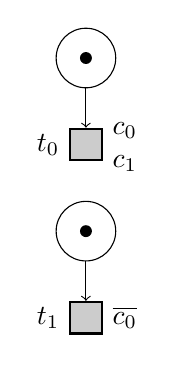
\begin{tikzpicture}

      % PLACES AND TRANSITIONS

      \node[place, tokens=1] (p0)  {};
      \node[transition, anchor=north] (t0) at ($(p0.south)-(0,.5)$) {};
      \node[place, tokens=1, anchor=north] (p1) at ($(t0.south)-(0,0.5)$) {};
      \node[transition, anchor=north] (t1) at ($(p1.south)-(0,.5)$) {};
      
      % LABELS

      \node[anchor=east] at ($(t0.west)$) {$t_0$};
      \node[anchor=east] at ($(t1.west)$) {$t_1$};
      
      % ARCS
      
      \draw[->] ($(p0.south)$) -- ($(t0.north)$);
      \draw[->] ($(p1.south)$) -- ($(t1.north)$);

      % CONDITIONS
      \node[anchor=west] at ($(t0.east)$) {
        \begin{tabular}{@{}l@{}}
          $c_0$ \\
          $c_1$ \\
        \end{tabular}
      };

      \node[anchor=west] at ($(t1.east)$) { $\overline{c_0}$};      
    \end{tikzpicture}
  };

  % Output design
  \node (design) [draw, rectangle, inner sep=1mm] at ($(pn.east)+(4,0)$) {
    \hspace*{20pt}    
    \begin{tikzpicture}
            
      % TDI idt0
      
      \draw       
      node [dipchip, num pins=4, hide numbers,
      no topmark, external pins width=0, anchor=south east]
      (idt0) {
        
      };

      \node[anchor=south] at ($(idt0.north)$) {$\gamma(t_0)$};

      \draw ($(idt0.bpin 1)$)
      node [anchor=west, font=\ssmall]  {\tt ic(0)};
      \draw ($(idt0.bpin 2)$)
      node [anchor=west, font=\ssmall]  {\tt ic(1)};

      % TDI idt1
      
      \draw       
      node [dipchip, num pins=4, hide numbers,
      no topmark, external pins width=0, anchor=north]
      (idt1) at ($(idt0.south)-(0,1)$) {
        
      };

      \node[anchor=south] at ($(idt1.north)$) {$\gamma(t_1)$};

      \draw ($(idt1.west)$)
      node [anchor=west, font=\ssmall, inner sep=1mm]  {\tt ic(0)};

      % INTERCONNECTIONS

      % \draw[red,->-=.5] ($(idt0.east)$) --++(.3,0)  |- ($(actionsps.west)+(0,.3)$) node[midway, yshift=-5pt, font=\ssmall] {$id_{m_0}$};
      % \draw[red,->-=.5] ($(idt1.east)$) --++(.3,0)  |- ($(actionsps.west)-(0,.3)$) node[midway, xshift=-8pt, font=\ssmall] {$id_{m_1}$};
      % \draw[red,->-=.5] ($(idt0.bpin 3)$) --++(.3,0) |- ($(idt1.bpin 1)$);
      % \draw[red,-<-=.5] ($(idt0.bpin 1)$) -|++ (-.3, 1.7) -| ($(idt0.east)+(.3,0)$) -- (idt0.east);
      % \draw[red,-<-=.5] ($(idt0.bpin 2)$) -|++ (-.3, -1.2) -| ($(idt1.east)+(.3,0)$) -- (idt1.east);
      
    \end{tikzpicture}

  }; 

  % CONDITION INPUT PORTS
  
  \draw[red, ->-=.5] ($(design.160)-(.3,0)$) --++ (1, 0)
  node[near start, above, anchor=south east] { $\gamma(c_1)$ }
  |- ($(idt0.bpin 1)$);
  \draw[red, ->-=.6] ($(design.200)-(.3,0)$) --++ (1, 0) coordinate (a)
  node[near start, above, anchor=south east] { $\gamma(c_0)$ }
  |- ($(idt0.bpin 2)$);
  \draw[red, ->-=.5] (a) |- ($(idt1.west)-(.1,0)$) node[anchor=west, draw, black, circle, fill=white, inner sep=1pt] {};
  
  % TRANSLATION ARROW
  
  \node at ($(pn.east)!.3!(design.west)$) {\Huge$\rightarrow$};
  
\end{circuitikz}

\end{document}

%%% Local Variables:
%%% mode: latex
%%% TeX-master: t
%%% End:
